\chapter{Proceso de Construcción y Evaluación del \textit{Pipeline}} \label{cap:metodologia}

La finalidad principal de este trabajo es detectar de forma automática los errores que registran los logs de un servicio universitario, mediante modelos de lenguaje pequeños ejecutados en la propia infraestructura, y avisar a los responsables con una sugerencia de causa y solución. Para ello se construyó un \textit{pipeline} que lee los registros del servicio \texttt{ms-users} de la DTIC, los reduce y agrupa en lotes, los clasifica con un SLM y reacciona ante los lotes con error. Como no existían etiquetas que dijeran qué registros eran errores, una parte central del trabajo fue construir esa referencia antes de poder evaluar cualquier modelo.

Este capítulo comienza describiendo el diseño general del sistema. Luego detalla el conjunto de datos y la construcción del \textit{ground truth}, que es la referencia contra la que se mide todo lo demás. Posteriormente explica la arquitectura del \textit{pipeline}, los modelos evaluados, la caché semántica y el ajuste fino con LoRA, y cierra con el diseño de la evaluación, la simulación en flujo continuo con errores inyectados y los mecanismos de notificación y recomendación.

\section{Diseño conceptual del sistema}\label{sec:met_vision}

El sistema se concibió como una cadena de etapas por la que pasa cada evento de log desde que el servicio lo escribe hasta que, si corresponde, llega una alerta a los responsables. En la figura~\ref{fig:arquitectura} se muestra el diseño general, que se organiza en cuatro bloques.

El primer bloque corresponde a los datos: los archivos o el flujo de logs del servicio se leen, se filtran para conservar solo los eventos con valor diagnóstico, se enmascaran sus partes variables y se agrupan en lotes de $N$ eventos consecutivos. El segundo bloque es el \textit{ground truth}, la referencia de qué lotes contienen un error, que se construyó una sola vez con tres LLM, revisión experta y reglas de propagación. El tercer bloque es la clasificación: cada lote se envía a un SLM, que responde si contiene un error, y opcionalmente una caché semántica evita consultar al modelo cuando el lote o sus eventos ya se conocen. El cuarto bloque es la reacción: los lotes con error disparan una alerta, un modelo separado redacta una recomendación, y un \textit{dashboard} muestra el estado de la ejecución y permite inyectar errores simulados.

\begin{figure}[H]
\centering
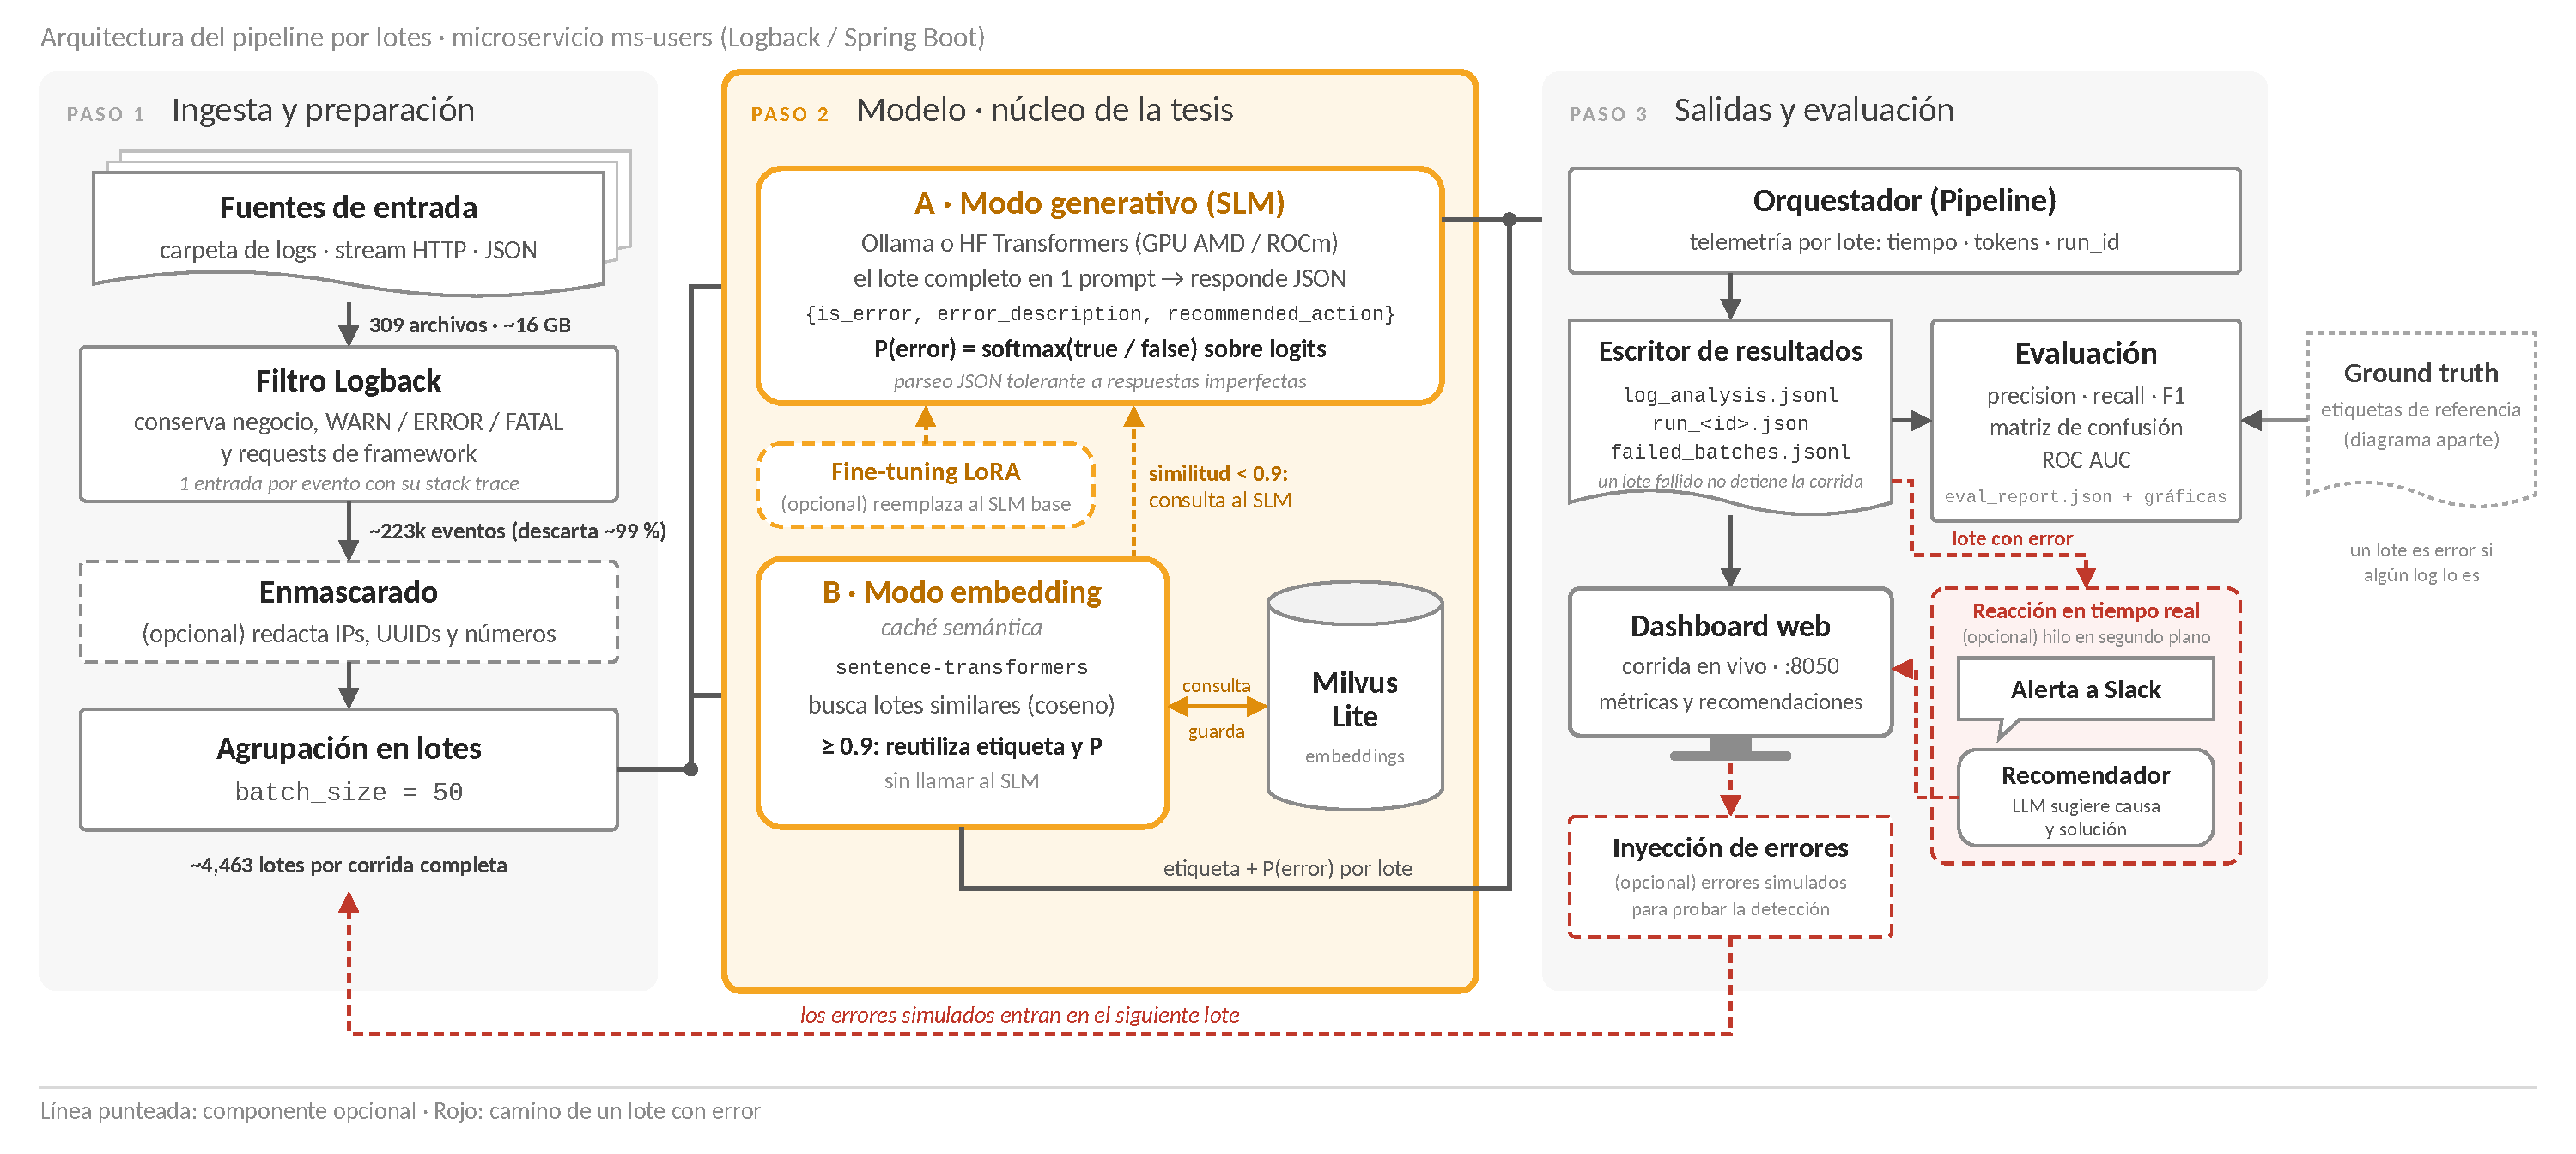
\includegraphics[width=\textwidth]{figs/metodologia/arquitectura_pipeline_completo_v2.pdf}
\caption{Diseño general del \textit{pipeline}: datos, \textit{ground truth}, clasificación y reacción.}
\label{fig:arquitectura}
\end{figure}

El sistema se usó de dos maneras. En la evaluación por lotes, el \textit{pipeline} recorrió el corpus histórico completo y cada respuesta se comparó con el \textit{ground truth}; así se evaluaron los modelos, los tamaños de lote y el ajuste fino. En la simulación en flujo continuo, un servidor local emitió los logs como si fueran el tráfico real del servicio, con errores inyectados en momentos conocidos, y el \textit{pipeline} los analizó en tiempo real; así se midieron la detección, la latencia, la dependencia del modelo y el uso de recursos.

\section{Conjunto de datos}\label{sec:met_dataset}

Los datos del trabajo provienen de \texttt{ms-users}, un microservicio Spring Boot de la DTIC que gestiona las cuentas de usuario de la universidad frente a Active Directory, LDAP, Oracle, AS400 y Google Workspace. Se dispuso de 309 archivos en formato Logback, con unos 16~GB y 27\,752\,836 eventos, que cubren del 23 de septiembre al 7 de octubre de 2026. El servicio rota su archivo de log al alcanzar unos 50~MB, lo que en la práctica equivale a un archivo por hora aproximadamente: cada día tiene entre 21 y 22 archivos numerados desde \texttt{logFile.AAAA-MM-DD.0.log}, salvo el 7 de octubre, que llega hasta el archivo \texttt{.7}, y el conjunto se completa con el archivo activo \texttt{logFile.log}, que termina a las 09:37 de ese día. Estos registros, generados por el servicio entre el 23 de septiembre y el 7 de octubre, fueron entregados para su uso en este trabajo por el director de la DTIC el 13 de octubre de 2026; a partir de esa fecha, la construcción del conjunto de datos y de su \textit{ground truth} se extendió hasta el 4 de noviembre.

\subsection{Características del corpus}

Casi todo el volumen del corpus es ruido de infraestructura: entre el 99.8\,\% y el 99.9\,\% corresponde a salida repetitiva que no describe operaciones del negocio. Las fuentes principales de ese ruido son los sondeos de salud de Kubernetes a \texttt{/actuator}, que Spring Security rechaza e imprime con trazas de pila de unas 115 líneas, las trazas internas de los filtros de Spring Security en nivel \texttt{TRACE} y las líneas de peticiones del \textit{framework}. Los eventos con valor de negocio son una fracción mínima y registran situaciones como rechazos por política de contraseñas, usuarios no encontrados en alguno de los sistemas externos, avisos de LDAP o cambios de contraseña exitosos.

\subsection{Prefiltrado y enmascarado}\label{subsec:met_prefiltro}

Para reducir el volumen se implementó un prefiltro basado en reglas que analiza cada evento Logback y decide si conservarlo según su \textit{logger}, su nivel de severidad y su mensaje, y nunca según la dirección IP. Se conservan los eventos de los \textit{loggers} de negocio, los de nivel \texttt{WARN}, \texttt{ERROR} o \texttt{FATAL} y las peticiones del \textit{framework}. Cada evento conservado forma una entrada cuyo texto es la línea original más su traza de pila, limitada a 15 líneas. El prefiltro conservó entre el 0.18\,\% y el 3.75\,\% de cada archivo, 223\,104 eventos en total, de los cuales solo unos 7\,400 son distintos.

Antes de que cualquier modelo vea el texto, las direcciones IP, los identificadores UUID y los números se sustituyen por marcadores. El enmascarado cumple dos funciones: evita que los identificadores salgan del texto que procesan los modelos y hace que los eventos repetidos, que solo difieren en esos valores, se vuelvan idénticos.

\subsection{Agrupación en lotes}\label{subsec:met_batches}

La unidad de análisis es el lote de $N$ eventos consecutivos ya filtrados. Para elegir $N$ se compararon cuatro tamaños con las etiquetas por evento disponibles en ese momento, midiendo qué proporción de lotes contendría un error y con qué frecuencia una ráfaga de errores consecutivos quedaría partida entre dos lotes. En la tabla~\ref{tab:met_tamano_lote} se muestran los resultados.

\begin{table}[H]
\centering
\caption{Comparación de tamaños de lote con las etiquetas por evento previas al criterio final.}
\label{tab:met_tamano_lote}
\small
\begin{tabular}{@{}rrrr@{}}
\toprule
$N$ & \textbf{Lotes} & \textbf{Lotes con error} & \textbf{Ráfagas de errores partidas} \\
\midrule
10 & 22\,311 & 9.4\,\% & 11.3\,\% \\
20 & 11\,156 & 16.1\,\% & 6.2\,\% \\
50 & 4\,463 & 30.8\,\% & 2.3\,\% \\
100 & 2\,232 & 46.0\,\% & 1.5\,\% \\
\bottomrule
\end{tabular}
\normalsize
\end{table}

Se eligió $N = 50$ como compromiso entre cuatro factores. El primero es la integridad de los errores: con lotes más pequeños, una ráfaga de errores queda partida entre dos lotes con más frecuencia (11.3\,\% con $N = 10$ frente a 2.3\,\% con $N = 50$), y el modelo ve solo una parte del incidente. El segundo es el costo computacional: un lote de 50 eventos ocupa una mediana de 4\,069 \textit{tokens} y un máximo de 5\,229 con el tokenizador del modelo de \textit{embeddings}, de modo que cabe holgadamente en la ventana de contexto de los modelos, mientras que con $N = 100$ la mediana sube a unos 8\,140 \textit{tokens} y el máximo a unos 9\,360, de modo que 524 de los 2\,232 lotes (23.5\,\%) superan el límite de 8\,192 \textit{tokens} del modelo de \textit{embeddings}, y con el tokenizador de Qwen3.5-9B lo superan 1\,377 lotes (61.7\,\%). En la práctica, los equipos de desarrollo no lograron procesar lotes de ese tamaño. El tercero es la latencia: al ritmo real del servicio, de unos 0.2 eventos por segundo (223\,104 eventos en 309 horas), un lote de 50 eventos tarda unos 250 segundos en llenarse, y un error que aparece en una posición al azar espera en promedio la mitad de ese tiempo antes de poder analizarse; con $N = 100$ esa espera se duplicaría. El cuarto es el número de llamadas al modelo, que crece al reducir el lote: con $N = 20$ se necesitan 2.5 veces más llamadas que con $N = 50$, y la evaluación de la sección~\ref{sec:met_evaluacion} no mostró una ventaja que lo compense (Capítulo~\ref{cap:resultados}). Con $N = 50$ el corpus se divide en 4\,463 lotes, 4\,462 de 50 eventos y uno final de 4. Los tamaños $N = 30$ y $N = 20$ se usaron después para medir el efecto del tamaño de lote sobre los modelos (sección~\ref{sec:met_evaluacion}).

La comparación anterior no incluía un tamaño intermedio entre 50 y 100, de modo que se hizo además una prueba de viabilidad con $N = 70$. Sobre los mismos 7\,000 primeros eventos del corpus, con $N = 50$ (140 lotes) y $N = 70$ (100 lotes), se ejecutaron tres modelos de la matriz en el equipo con 8~GB de memoria de GPU. La prueba midió si los modelos podían responder, y no la calidad de su detección. En la tabla~\ref{tab:met_n70} se muestran los resultados; los \textit{tokens} incluyen la entrada y la salida de cada llamada.

\begin{table}[H]
\centering
\caption{Prueba de viabilidad con $N = 50$ y $N = 70$ sobre los primeros 7\,000 eventos.}
\label{tab:met_n70}
\small
\begin{tabular}{@{}p{3.3cm}cp{1.8cm}p{2.6cm}p{1.6cm}p{1.6cm}@{}}
\toprule
\textbf{Modelo} & $N$ & \textbf{Respuestas válidas} & \textbf{\textit{Tokens} por lote (mediana / máx.)} & \textbf{\textit{Tokens} por evento} & \textbf{s por lote (mediana)} \\
\midrule
SmolLM2-1.7B-Instruct & 50 & 130 / 140 & 5\,380 / 5\,888 & 108.0 & 2.0 \\
 & 70 & 1 / 100 & 7\,625 / 8\,269 & 109.1 & 8.5 \\
Ministral-3-3B (BF16) & 50 & 140 / 140 & 4\,488 / 4\,757 & 89.7 & 13.8 \\
 & 70 & 100 / 100 & 6\,172 / 6\,692 & 87.9 & 16.0 \\
Qwen3.5-9B (Q6\_K) & 50 & 140 / 140 & 4\,327 / 4\,609 & 86.7 & 5.2 \\
 & 70 & 100 / 100 & 6\,005 / 6\,502 & 85.9 & 6.7 \\
\bottomrule
\end{tabular}
\normalsize
\end{table}

De la prueba se desprenden cuatro argumentos. El primero es que el tamaño de lote lo limita el modelo con la ventana de contexto más pequeña, y una matriz comparable exige el mismo $N$ para todos los modelos. Ese modelo es SmolLM2-1.7B, con una ventana de 8\,192 \textit{tokens}, que es además el modelo con el que se desarrolló y probó el \textit{pipeline} desde el inicio y que se usa como referencia. Con $N = 50$ cabe en su ventana (en el corpus completo, el lote más largo ocupa 7\,648 \textit{tokens} y solo el 2.9\,\% de sus respuestas son inválidas), pero con $N = 70$ el lote mediano ya ocupa 7\,625 \textit{tokens}, el 93\,\% de la ventana, y 99 de 100 respuestas salieron en prosa y no en JSON; con ellas desapareció también la acción recomendada, que el modelo devolvió en 130 de los 140 lotes con $N = 50$ y en ninguno con $N = 70$. El segundo es que la degradación empieza antes de llegar al límite: la mediana con $N = 70$ queda por debajo de 8\,192 \textit{tokens} y aun así casi todas las respuestas fallaron, y en la ejecución completa con $N = 50$ los lotes con respuesta inválida son más largos (mediana de 6\,356 \textit{tokens} frente a 5\,645 del total), lo que indica que la tasa de fallos crece con la longitud del lote. El tercero es que $N = 70$ no ahorra \textit{tokens}: el total por evento es casi igual en ambos tamaños, y solo se reduce el número de llamadas, a cambio de que cada una sea unas 1.4 veces más grande y más lenta (16\,\% más en Ministral, 29\,\% más en Qwen3.5-9B y unas cuatro veces más en SmolLM2). El cuarto es que $N = 70$ no encaja con el \textit{ground truth}: la revisión experta, las reglas y la propagación se hicieron por lotes de 50, y como 70 no es múltiplo de 50, evaluarlo con etiquetas exactas exigiría bloques de 350 eventos o rehacer la votación y la revisión.

Ministral-3-3B y Qwen3.5-9B sí respondieron sin fallos con $N = 70$, y no se midió si ese tamaño mejora o empeora su detección. La prueba respalda, por tanto, que $N = 70$ no es viable para toda la matriz de modelos, y no que $N = 50$ sea mejor para cada modelo. Su alcance es limitado: usa 7\,000 eventos y un solo equipo, y no considera la memoria de GPU como evidencia, porque Ollama reserva la misma memoria con ambos tamaños.

\section{Construcción del \textit{ground truth}}\label{sec:met_gt}

No existían etiquetas que indicaran qué eventos del corpus eran errores, de modo que la referencia se construyó por etapas que combinaron el pseudoetiquetado con modelos de lenguaje y la revisión de expertos. Se decidió que el \textit{ground truth} fuera por lote y no por evento, porque un SLM evalúa un lote completo y su respuesta debe compararse con una etiqueta del mismo nivel. En la figura~\ref{fig:met_gt} se resume el proceso.

\figpendiente{fig:met_gt}{Etapas de la construcción del \textit{ground truth}.}{Diagrama de flujo: etiquetado por evento con tres LLM $\rightarrow$ votación por lote $\rightarrow$ muestra estratificada de 220 lotes $\rightarrow$ revisión experta y criterio operativo $\rightarrow$ propagación por reglas y similitud $\rightarrow$ rondas dirigidas $\rightarrow$ \textit{ground truth} final (130 lotes con error).}

\subsection{Etiquetado de cada evento}

En una primera etapa, tres LLM locales de 7\,000 a 8\,000 millones de parámetros, de familias distintas (Qwen2.5-7B, Llama3.1-8B y Mistral-7B, servidos con Ollama), etiquetaron por separado cada uno de los 223\,104 eventos en siete categorías: normal, autenticación o política, usuario no encontrado, fallo de \textit{backend}, excepción de aplicación, actividad sospechosa y error genérico. El voto mayoritario marcó como error 4\,738 eventos (2.12\,\%), con un acuerdo alto entre los tres anotadores ($\kappa$ de Fleiss de 0.89) \cite{fleiss1971_kappa}. Estas etiquetas por evento sirvieron para elegir el tamaño de lote, pero no se reutilizaron como referencia final.

\subsection{Votación por lote}\label{subsec:met_votacion}

Los mismos tres modelos votaron después sobre cada lote completo de 50 eventos. Cada uno recibió el lote como una lista numerada y devolvió un veredicto único en JSON con tres campos: si el lote contiene un error, los índices de las líneas que lo justifican y una frase de razonamiento. Un lote se consideró error si contenía al menos un evento erróneo, y un lote sin respuesta válida no se etiquetó, en lugar de asumirlo normal, para no sesgar el voto. Los modelos se ejecutaron con cuantización Q4\_K\_M, temperatura 0, una ventana de contexto de 12\,288 \textit{tokens}, un máximo de 300 \textit{tokens} de respuesta y tres reintentos; ningún lote se truncó. El \textit{prompt} completo se incluye en el Anexo~\ref{ap:prompt_votacion}, y en la tabla~\ref{tab:met_votos} se resume la votación.

\begin{table}[H]
\centering
\caption{Votación de los tres LLM sobre los 4\,463 lotes de 50 eventos.}
\label{tab:met_votos}
\small
\begin{tabular}{@{}lrrr@{}}
\toprule
\textbf{Modelo} & \textbf{Lotes con voto de error} & \textbf{Tiempo total (h)} & \textbf{\textit{Tokens} de entrada (mediana / máx.)} \\
\midrule
qwen2.5:7b & 1\,304 & 3.7 & 4\,595 / 5\,767 \\
llama3.1:8b & 1\,396 & 2.3 & 3\,716 / 4\,836 \\
mistral:7b & 1\,400 & 4.5 & 5\,544 / 6\,942 \\
\bottomrule
\end{tabular}
\normalsize
\end{table}

Durante la votación, Mistral dejó 23 lotes sin voto porque cortaba el JSON sin cerrar la comilla ni la llave final, y como la salida con temperatura 0 es determinista, los reintentos repetían el mismo fallo. Se agregó al analizador de respuestas un rescate mediante expresiones regulares y los 23 lotes se reprocesaron.

\subsection{Consenso entre modelos}\label{subsec:met_kappa}

El consenso se definió como la mayoría estricta sobre los votos válidos, es decir, al menos dos de los tres modelos. Con esa regla, 1\,370 lotes (30.7\,\%) resultaron error y 3\,093 normales. El acuerdo entre los modelos fue alto: el $\kappa$ de Fleiss fue 0.886, interpretado como casi perfecto según la escala de Landis y Koch \cite{landis1977_kappa}, con 1\,203 lotes de error unánime, 2\,936 de normal unánime y 324 con desacuerdo. Este consenso se trató solo como una etiqueta preliminar, que sirvió para guiar la revisión experta.

\subsection{Revisión experta y criterio operativo}\label{subsec:met_expertos}\label{sec:met_criterio}

Para contrastar el consenso con el criterio humano se extrajo una muestra aleatoria estratificada de 220 lotes, alrededor del 5\,\% del total, con semilla 42 y el reparto de 88 lotes de error unánime, 88 de desacuerdo y 44 de normal unánime. Los dos revisores se dividieron la muestra en dos mitades de 110 lotes sin solapamiento, con la misma mezcla de estratos, y marcaron cada lote como error o normal viendo las líneas señaladas por los modelos, sus razonamientos y el texto completo del lote.

En la primera revisión, cada revisor aplicó su propio criterio y ambos contradijeron al consenso en el 37.5\,\% de los lotes de error unánime y en el 27.3\,\% de los de desacuerdo, y en ninguno de los de normal unánime. Los modelos marcaban como error condiciones que la institución considera normales. Por ello, los revisores se reunieron y acordaron el criterio operativo de la tabla~\ref{tab:met_criterio}, que distingue las fallas del sistema de las condiciones funcionales que el servicio maneja correctamente.

\begin{table}[H]
\centering
\caption{Criterio operativo de error acordado por los revisores.}
\label{tab:met_criterio}
\small
\begin{tabular}{@{}p{7.2cm}p{7.2cm}@{}}
\toprule
\textbf{Es error (falla del sistema)} & \textbf{Es normal (condición funcional manejada)} \\
\midrule
Respuestas HTTP 5xx & Respuestas HTTP 4xx del cliente \\
Excepciones no controladas de la aplicación & Usuario no encontrado en AD, Google, LDAP u Oracle, y siempre en AS400 (decisión explícita) \\
Fallos al crear o actualizar cuentas por causa interna & Rechazo por política de contraseñas \\
Fallas de la API de AD o de conectividad & Entidades que ``ya existen'' \\
Errores de base de datos o del \textit{pool} de conexiones, fallo al iniciar el servicio y correo no enviado & Operaciones exitosas \\
\bottomrule
\end{tabular}
\normalsize
\end{table}

Con este criterio se volvieron a etiquetar los 220 lotes: 63 etiquetas pasaron de error a normal y ninguna de normal a error. Solo el 12.5\,\% de los lotes de error unánime (11 de 88) resultaron error según los expertos, frente al 6.8\,\% de los de desacuerdo y al 0\,\% de los de normal unánime. Como esta es la única muestra aleatoria del proceso, es la que permite estimar tasas sobre el corpus completo.

\subsection{Propagación del criterio experto}\label{subsec:met_propagacion}

Revisar los 4\,463 lotes no era viable, de modo que el criterio experto se extendió al resto de forma reproducible y registrando el origen de cada etiqueta. Para cada lote se aplicaron, en orden, las siguientes reglas, y decidió la primera que se cumplía. Si un experto lo había revisado, se usó su etiqueta. Si ningún LLM había votado error, el lote se etiquetó como normal, una regla que la muestra respalda, porque ninguno de los 44 lotes de normal unánime fue contradicho. Si algún evento cumplía una regla de error (respuestas 5xx, el mensaje ``Failed to complete request'', errores al crear o actualizar cuentas o errores de la API de AD, con exclusiones para ``ya existe'' y la política de contraseñas), el lote se etiquetó como error. Si todo lo señalado por los modelos era ``usuario no encontrado'' de AS400, el lote fue normal. Por último, si el lote se parecía a lotes ya revisados, heredó su etiqueta cuando había una mayoría clara; la similitud se midió con el índice de Jaccard entre los tipos de evento señalados por los LLM, con un umbral de 0.5 y una pureza mínima de 0.8.

Si ninguna regla aplicaba, el lote no se completó con el voto de los LLM, sino que pasó a revisión. Así se hicieron tres rondas dirigidas, con 91, 17 y 1 representantes de grupos de lotes idénticos que cubrieron 110, 22 y 1 lotes. En total, los expertos revisaron 329 lotes (7.4\,\%), de los cuales 39 resultaron error y 290 normales.

\subsection{\textit{Ground truth} final}

El resultado es una etiqueta para cada uno de los 4\,463 lotes, sin ninguno pendiente. En la tabla~\ref{tab:met_origen} se muestra el origen de las etiquetas. Los 130 lotes con error (2.9\,\%) provienen solo de la revisión directa (39) y de las reglas de error (91); la similitud con lotes revisados únicamente asignó etiquetas normales. Frente al consenso de los LLM, los expertos eliminaron 1\,241 de sus 1\,370 positivos y añadieron un error nuevo, y ambas referencias coinciden solo en el 72.2\,\% de los lotes. Esta etiqueta, denominada \texttt{final\_is\_error}, es la referencia de todas las evaluaciones del trabajo.

\begin{table}[H]
\centering
\caption{Origen de las etiquetas del \textit{ground truth} final por lote ($N=50$).}
\label{tab:met_origen}
\small
\begin{tabular}{@{}lr@{}}
\toprule
\textbf{Origen} & \textbf{Lotes} \\
\midrule
Ningún LLM votó error & 2\,892 \\
Similitud con un lote revisado & 1\,093 \\
Revisión experta & 329 \\
Regla de error & 91 \\
Regla de AS400 (normal) & 58 \\
\midrule
\textbf{Total} & \textbf{4\,463} \\
\bottomrule
\end{tabular}
\normalsize
\end{table}

La diferencia entre el voto de los LLM y el criterio experto muestra la dificultad central del problema: un modelo genérico interpreta cualquier excepción o línea de nivel \texttt{ERROR} como una falla, mientras que la institución considera muchas de ellas resultados normales del negocio.

\section{Arquitectura del \textit{pipeline}}\label{sec:met_arquitectura}

Sobre los datos ya preparados, el \textit{pipeline} se implementó en Python como una cadena de componentes intercambiables: un lector que entrega los eventos, un modelo que analiza cada lote y un escritor que registra cada resultado. Esta organización permitió usar el mismo flujo tanto sobre los archivos históricos como sobre un flujo HTTP en vivo, y cambiar el modelo o el tipo de caché sin modificar el resto.

\tema{Ingesta}

El lector obtiene los eventos de los archivos de log, en orden alfabético para que el orden sea reproducible, o de un flujo HTTP que simula la operación en vivo. A cada evento le aplica el prefiltro y el enmascarado descritos en la sección~\ref{subsec:met_prefiltro} y los agrupa en lotes de $N$ eventos conservados.

\tema{Clasificación}

Cada lote se envía al SLM como una lista numerada de eventos, acompañada de un mensaje de sistema fijo que define la tarea, el formato de respuesta y las condiciones que no deben considerarse error, como las solicitudes erróneas, las excepciones de validación de contraseñas o los usuarios no encontrados. El modelo responde un objeto JSON corto con tres campos: si hay error, una descripción breve y una acción recomendada. El mensaje de sistema completo se incluye en el Anexo~\ref{ap:prompt_slm}. Se implementaron dos motores de inferencia intercambiables: Ollama, para los modelos cuantizados en formato GGUF, y Hugging Face Transformers, para los modelos en su formato original. En ambos casos la decodificación fue determinista (temperatura 0 en Ollama y decodificación voraz en Transformers), con el razonamiento extendido de los modelos desactivado y un máximo de 512 \textit{tokens} de respuesta.

\tema{Probabilidad de error}

Además de la respuesta binaria, el \textit{pipeline} registra la probabilidad de error de cada lote, que se obtiene de las probabilidades que el modelo asigna a los \textit{tokens} \texttt{true} y \texttt{false} en la posición donde escribe su decisión (sección~\ref{sec:mt_probabilidad}). En Transformers se calcula a partir de los \textit{logits} y en Ollama a partir de las probabilidades logarítmicas de las alternativas más probables que devuelve el servidor. Esta puntuación permite construir las curvas ROC y de precisión-exhaustividad y elegir umbrales de decisión distintos de 0.5.

\tema{Robustez}

Los modelos pequeños no siempre respetan el formato pedido, de modo que se implementaron varias protecciones. Un analizador tolerante repara las respuestas mal formadas, como saltos de línea sin escapar, comillas sin cerrar, claves sin comillas o un JSON cortado, y en algunos modelos recuperó el 100\,\% de las respuestas que de otro modo se habrían perdido. Un registro de fallos guarda la entrada y la respuesta cruda de cada lote que no se puede procesar, sin detener la ejecución. Un límite de \textit{tokens} de salida y un tiempo máximo por petición detienen las generaciones descontroladas; en una ocasión, un modelo llegó a generar 141\,000 \textit{tokens} para un solo lote. Por último, una ejecución interrumpida se reanuda exactamente desde el primer lote que no llegó a escribirse.

\section{Modelos de lenguaje pequeños evaluados}\label{sec:met_slm}

Para el clasificador se seleccionaron ocho SLM de 1\,000 a 9\,000 millones de parámetros, de familias y desarrolladores distintos, ejecutados localmente y en su mayoría cuantizados. En la tabla~\ref{tab:met_modelos} se listan los modelos y el motor con que se ejecutó cada uno\falta{DATO: criterio con que se eligieron los ocho modelos (disponibilidad, licencia, tamaño en VRAM, familia), para justificar la selección}.

\begin{table}[H]
\centering
\caption{SLM evaluados como clasificadores.}
\label{tab:met_modelos}
\small
\begin{tabular}{@{}p{5.6cm}p{2.6cm}p{5.6cm}@{}}
\toprule
\textbf{Modelo} & \textbf{Motor} & \textbf{Formato} \\
\midrule
Qwen3.5-9B & Ollama & GGUF, cuantización Q6\_K \\
IBM Granite-4.1-3B & Transformers & Formato original \\
Microsoft Phi-3.5-mini (3.8B) & Transformers & Formato original \\
Google Gemma-3-4B & Transformers & Formato original \\
Ling-3.0-tiny & Ollama & GGUF, cuantización Q4\_K\_M \\
Ministral-3-3B & Ollama & GGUF, BF16 \\
Llama-3.2-1B \textit{log-analyzer} & Ollama & GGUF, cuantización Q4\_K\_M \\
SmolLM2-1.7B-Instruct & Transformers & Formato original \\
\bottomrule
\end{tabular}
\normalsize
\end{table}

Todos los modelos recibieron el mismo \textit{prompt}, el mismo enmascarado, el mismo presupuesto de salida y decodificación determinista, de modo que las diferencias entre ellos se deben solo al modelo. Dos modelos requirieron un tratamiento especial. El Llama-3.2-1B \textit{log-analyzer}, un ajuste público orientado a logs, solo funcionó a través de Ollama con su propia plantilla de conversación, porque con Transformers repetía los logs en lugar de responder. El modelo base SmolLM2-1.7B, sin ajuste para seguir instrucciones, solo respondió de forma válida en el 49\,\% de los lotes y se conservó únicamente como referencia.

\subsection{Entorno de desarrollo}\label{subsec:met_entorno}

El desarrollo y la experimentación se repartieron entre dos equipos con tarjetas gráficas de fabricantes distintos, por lo que el \textit{pipeline} admite tanto la plataforma ROCm de AMD como CUDA de NVIDIA. En la tabla~\ref{tab:met_equipos} se describen ambos equipos.

\begin{table}[H]
\centering
\caption{Equipos utilizados en el desarrollo y la experimentación.}
\label{tab:met_equipos}
\small
\begin{tabular}{@{}p{3cm}p{5.4cm}p{5.4cm}@{}}
\toprule
 & \textbf{Equipo 1} & \textbf{Equipo 2} \\
\midrule
GPU & AMD Radeon RX 7900 XT & NVIDIA GeForce RTX 4060 \\
VRAM & 20~GB & 8~GB \\
RAM & 24~GB & 16~GB \\
Sistema operativo & Debian & Ubuntu \\
Aceleración & ROCm 7.2 (PyTorch 2.13) & CUDA \\
Uso principal & Mayoría de clasificaciones, simulación y ajuste fino & Qwen3.5-9B y Ministral-3-3B con $N=30$; SmolLM2-1.7B con $N=50$ \\
\bottomrule
\end{tabular}
\normalsize
\end{table}

El \textit{pipeline} se escribió en Python 3.13, con Pydantic para las estructuras de logs, lotes y resultados. Los modelos se sirvieron con Ollama, ejecutado en un contenedor Docker, y con Hugging Face Transformers sobre PyTorch. Los \textit{embeddings} se generaron con Sentence-Transformers y se almacenaron en Milvus Lite. Las métricas se calcularon con scikit-learn, las pruebas estadísticas con NumPy y SciPy, y las gráficas con Matplotlib. El ajuste fino usó las bibliotecas PEFT y bitsandbytes, y llama.cpp para convertir el adaptador al formato de Ollama. El código se versionó con Git.

\subsection{Pruebas del software}\label{sec:met_pruebas}

Para asegurar que cada componente se comportara como se esperaba, el proyecto incluye 380 pruebas unitarias agrupadas en 39 conjuntos, todas superadas al cierre de este trabajo. Cubren, entre otros aspectos, el análisis de las respuestas de los modelos, el prefiltro, el cálculo de la probabilidad de error, la caché por evento, la construcción del \textit{ground truth} por lote, la reanudación de ejecuciones interrumpidas, las pruebas de significancia, el ajuste fino y la simulación.

\section{Caché semántica}\label{sec:met_cache}

Los logs del servicio se repiten mucho: entre los 223\,104 eventos conservados hay solo unos 7\,400 distintos. Esto sugiere que muchas consultas al modelo podrían evitarse reutilizando respuestas ya obtenidas, y para comprobarlo se implementó una caché opcional con tres variantes, que se compararon en la simulación (sección~\ref{sec:met_simulacion}).

\tema{Modelo de \textit{embeddings}}

Los textos se convierten en vectores con Qwen3-Embedding-0.6B \cite{zhang2025_qwen3emb}. Los vectores se truncan a 512 dimensiones aprovechando que el modelo admite representaciones \textit{Matryoshka} \cite{kusupati2022_matryoshka}, se vuelven a normalizar y se generan sin instrucción. El modelo se configuró con un límite de 8\,192 \textit{tokens}, de modo que tanto un evento, de unos 85 \textit{tokens}, como un lote completo de 50 eventos caben enteros sin truncarse. Cada vector de 512 dimensiones ocupa 2~KB y se almacena en Milvus Lite.

\tema{Caché por lote}

En esta variante, cada lote completo se convierte en un \textit{embedding} y se busca el lote guardado más parecido según la similitud del coseno (sección~\ref{sec:mt_embeddings}), que compara la dirección de los vectores con independencia de su magnitud. Si esa similitud supera un umbral, se reutiliza su respuesta sin llamar al SLM; si no, el SLM responde y el lote se guarda.

\tema{Caché por evento}

En esta variante la decisión se toma evento a evento, con dos estados. Un evento pasa a ser \emph{normal conocido} cuando aparece en un lote que el SLM respondió como normal. Si el SLM marca un lote como error, sus eventos todavía desconocidos quedan como \emph{sospechosos}, porque el modelo no indica qué línea contiene el error y se asume que está entre los eventos nuevos. Un lote evita al SLM solo si todos sus eventos son normales conocidos; cualquier evento desconocido o sospechoso lo envía al modelo, y un evento sospechoso que luego aparece en un lote normal pasa a normal. En la variante exacta, cada evento se compara por su texto enmascarado sin la marca de tiempo y las claves se guardan en memoria; en la variante por similitud, un evento nunca visto toma el estado del evento guardado más parecido si la similitud del coseno supera el umbral. En la figura~\ref{fig:met_cache_evento} se ilustra esta lógica.

\figpendiente{fig:met_cache_evento}{Lógica de decisión de la caché por evento.}{Diagrama de decisión: lote nuevo $\rightarrow$ ¿todos los eventos son normales conocidos? (sí: respuesta ``normal'' sin SLM) $\rightarrow$ (no) ¿hay eventos desconocidos? (sí: consultar al SLM y actualizar estados) $\rightarrow$ (no, solo sospechosos) vía rápida: alerta sin SLM. Indicar cómo cambia el estado de un evento (desconocido, normal conocido, sospechoso).}

\tema{Vía rápida}

La vía rápida extiende la caché por evento: si un lote no tiene eventos desconocidos y contiene al menos uno sospechoso, la alerta se emite directamente, sin llamar al SLM. Se probó en su variante exacta y con umbrales de similitud de 0.99 y 0.995.

\tema{Elección de los umbrales}

Los umbrales de similitud se eligieron antes de la simulación, reproduciendo las respuestas de Qwen3.5-9B sobre el corpus original de 4\,463 lotes y 130 errores. Se probaron, para la caché por lote, los umbrales 0.90, 0.95, 0.97, 0.98, 0.99 y 0.995, y para la caché por evento con similitud, 0.85, 0.90, 0.95, 0.97, 0.98, 0.99 y 0.995. El rango cubre desde casi no usar la caché hasta usarla casi siempre, y se descartaron los extremos sin interés: 0.999 en la caché por lote, que ya no evita llamadas, y 0.80 en la caché por evento, que pierde demasiados errores.

\section{Ajuste fino con LoRA}\label{sec:met_finetuning}

Las primeras evaluaciones mostraron que los SLM detectaban los errores reales, pero marcaban como error muchas condiciones que la institución considera normales. Para alinear el criterio del mejor modelo, Qwen3.5-9B, con el del \textit{ground truth} experto y reducir sus falsas alarmas, se le aplicó un ajuste fino con LoRA \cite{hu2022_lora}.

\subsection{Datos de entrenamiento, validación y prueba}

Los datos son los lotes de 50 eventos con su etiqueta \texttt{final\_is\_error}, presentados con el mismo \textit{prompt} y el mismo formato de respuesta JSON que usa el \textit{pipeline}. El corpus se dividió en el tiempo, por la posición de los lotes, con un lote de separación entre partes, para que la prueba simulara datos futuros y ningún texto de un lote de prueba apareciera en el entrenamiento. En la tabla~\ref{tab:met_particion} se muestra la partición.

\begin{table}[H]
\centering
\caption{Partición temporal del corpus para el ajuste fino.}
\label{tab:met_particion}
\small
\begin{tabular}{@{}llrr@{}}
\toprule
\textbf{Parte} & \textbf{Lotes del corpus} & \textbf{Ejemplos} & \textbf{Con error} \\
\midrule
Entrenamiento & 0--3\,123 (70\,\%) & 693 & 77 \\
Validación & 3\,125--3\,569 (10\,\%) & 224 & 24 \\
Prueba & 3\,571--4\,462 (20\,\%) & 892 (todos) & 29 \\
\bottomrule
\end{tabular}
\normalsize
\end{table}

El conjunto de entrenamiento no incluye todos los lotes de su tramo. Se tomaron los 77 lotes con error, 423 negativos difíciles y 193 negativos fáciles, en una proporción de ocho negativos por cada error. Los negativos difíciles son lotes normales que el modelo sin ajustar marcaba como error, es decir, sus propias falsas alarmas, que son justamente el comportamiento que se buscaba corregir. La validación incluye los 24 errores de su tramo y 200 lotes normales, y la prueba conserva todos los lotes de su tramo para medir el desempeño con la prevalencia real.

\subsection{Configuración del entrenamiento}

Se aplicó QLoRA \cite{dettmers2023_qlora}: el modelo base Qwen3.5-9B se cargó cuantizado a 4 bits con NormalFloat (NF4), a partir de una copia ya cuantizada para no agotar la memoria RAM, y se entrenó un adaptador LoRA de rango 16, $\alpha = 32$ y \textit{dropout} de 0.05 en todas las capas lineales, con unos 43 millones de parámetros entrenables, el 0.48\,\% del modelo. La pérdida se ponderó para compensar el desbalance de clases: los ejemplos con error pesan 4 veces, los negativos difíciles 2 veces y el \textit{token} de decisión (\texttt{true} o \texttt{false}), 10 veces, porque es el que determina la clasificación. Se entrenó con una tasa de aprendizaje de $10^{-4}$, durante dos épocas, con acumulación de gradientes de 8 ejemplos (174 pasos) y hasta 6\,144 \textit{tokens} por ejemplo. Cada 20 pasos se validó el modelo y se guardó un punto de control desde el que el entrenamiento podía reanudarse tras un corte, y se conservó el de menor pérdida de validación.

El entrenamiento se ejecutó en el equipo 1 y duró 10.6 horas, con un máximo de 19.1~GiB de memoria de GPU. Un primer intento se perdió por un apagado del equipo, lo que motivó el guardado periódico de puntos de control. La pérdida de validación bajó de 0.239, tras el primer cuarto de época, a un mínimo de 0.166 en la época 1.6, y se mantuvo estable hasta el final (0.167).

\subsection{Despliegue del modelo ajustado}

El adaptador se convirtió al formato GGUF con llama.cpp, con un tamaño de 86~MB, y un archivo de configuración de Ollama lo aplica sobre el mismo Qwen3.5-9B Q6\_K usado en todas las evaluaciones. De este modo, la comparación entre el modelo base y el ajustado cambia solo el adaptador. El modelo ajustado clasificó el corpus completo con la misma configuración que el modelo base: 4\,463 lotes en 3.5 horas, unos 2.8 segundos por lote, sin respuestas inválidas.

\section{Diseño de la evaluación}\label{sec:met_evaluacion}

La evaluación buscó responder tres preguntas: qué modelo detecta mejor los errores, cuánto influye el tamaño del lote y si el ajuste fino mejora al modelo base. Para que las diferencias se debieran solo al modelo y al tamaño de lote, todas las ejecuciones usaron el mismo filtro, el mismo enmascarado y el mismo \textit{prompt}.

\subsection{Matriz de tamaños de lote}

Cada modelo procesó el corpus completo con tres tamaños de lote: $N = 50$ (4\,463 lotes), $N = 30$ (7\,437 lotes) y $N = 20$ (11\,156 lotes). Así se midió si dar al modelo más o menos contexto por decisión mejora o empeora su desempeño.

\subsection{Métricas}\label{subsec:met_metricas}

Cada lote del modelo se comparó con el lote correspondiente del \textit{ground truth} y se calcularon la precisión, la exhaustividad, el $F_1$, la exactitud, la exactitud balanceada, la especificidad, el MCC y el AUC de la curva ROC, junto con las matrices de confusión y las curvas ROC y de precisión-exhaustividad (sección~\ref{sec:mt_metricas}). La curva de precisión-exhaustividad recorre todos los umbrales sobre la probabilidad de error y se resume con la precisión promedio (AP), cuya referencia es la de un clasificador al azar, igual a la proporción de errores (0.029 con $N = 50$). Como solo el 2.9\,\% de los lotes son errores, la exactitud resulta engañosa, y los criterios principales fueron el MCC, la exactitud balanceada y la precisión \cite{chicco2020_mcc}.

\figpendiente{fig:met_pr_ejemplo}{Ejemplo de curva de precisión-exhaustividad con la referencia del clasificador al azar.}{Opcional: curva PR de un modelo con la línea horizontal en 0.029 (clasificador al azar), para ilustrar la lectura de la AP. Puede omitirse si las curvas del Capítulo~\ref{cap:resultados} ya lo muestran.}

\subsection{Evaluación por similitud para $N = 30$ y $N = 20$}

El \textit{ground truth} experto existe solo para lotes de 50 eventos, de modo que un lote de 30 o de 20 no tiene una etiqueta propia. Para evaluarlos, cada lote de 30 o de 20 recibió la etiqueta del lote de 50 del \textit{ground truth} más parecido, y la respuesta del SLM se comparó con esa etiqueta prestada. Los lotes se convirtieron en \textit{embeddings} con el mismo modelo de la caché, completos y sin truncar, y se tomó el vecino más cercano por similitud del coseno ($k = 1$). La referencia se calculó con los lotes de Qwen3.5-9B, que respondió a todos, ya que el texto de un lote es el mismo para todos los modelos con el mismo $N$.

Este procedimiento se validó de dos formas. Aplicado a los propios lotes de 50, el vecino fue siempre el mismo lote, con similitud 1, y se reprodujeron exactamente las métricas de la evaluación directa, lo que confirmó que la alineación y los \textit{embeddings} eran correctos. Además, la etiqueta prestada coincidió en el 97.7\,\% de los lotes con la del lote de 50 que contiene los mismos eventos. Los lotes cuya referencia es error resultaron los menos parecidos a su vecino, porque los errores son el texto menos común, de modo que su etiqueta prestada es la menos segura. Al exigir una similitud mínima, los lotes con error eran los primeros en quedar fuera, por lo que el resultado principal usa todos los lotes y la similitud se reporta solo como control. Las cifras de $N = 30$ y $N = 20$ sirven, por tanto, para comparar modelos dentro de un mismo tamaño de lote y no para compararlas directamente con las de $N = 50$.

\subsection{Significancia estadística}\label{subsec:met_significancia}

Para saber si las diferencias entre modelos eran reales o fruto del azar se aplicó un procedimiento en dos pasos. En el primero, para cada métrica, una prueba de permutación pareada entre todos los modelos contrastó la hipótesis nula de que todos rinden igual\falta{fuente de la prueba de permutación pareada (p. ej. Good, ``Permutation, Parametric and Bootstrap Tests of Hypotheses'', Springer, 2005)}. En cada una de las 10\,000 permutaciones se intercambiaron al azar las predicciones de los modelos dentro de cada lote, y el estadístico fue la diferencia entre el mejor y el peor valor de la métrica. En el segundo paso, solo para las métricas en que se rechazó la hipótesis global, se compararon los modelos por pares con la misma prueba. Como se probaron muchas métricas y pares a la vez, los valores $p$ se corrigieron con el procedimiento de Holm \cite{holm1979_sequential}.

Los lotes en que un modelo no dio una respuesta válida se contaron como fallos de ese modelo: falso negativo si el lote tenía un error y falso positivo si era normal, con la peor probabilidad posible para el AUC. Así cada modelo se evaluó sobre todos los lotes, en lugar de quitar un lote a todos cuando uno solo fallaba en él. Los intervalos de confianza del 95\,\% se calcularon con un \textit{bootstrap} circular por bloques de 2\,000 remuestreos, que remuestrea tramos de lotes consecutivos en lugar de lotes sueltos, porque los lotes vecinos están correlacionados\falta{fuente del bootstrap por bloques (p. ej. Künsch, ``The jackknife and the bootstrap for general stationary observations'', Annals of Statistics, 1989) y de la regla de la raíz cúbica para la longitud del bloque}; la longitud de los bloques se fijó en la raíz cúbica del número de lotes.

\subsection{Evaluación del ajuste fino}

El modelo ajustado y el modelo base se compararon solo sobre los 892 lotes de prueba, con 29 errores; los lotes de entrenamiento no se calificaron, y los de validación solo sirvieron para elegir el umbral. Para cada modelo se evaluaron dos variantes: su respuesta tal cual y una variante con umbral, que marca error cuando la probabilidad de error supera el umbral que maximiza el MCC en los 445 lotes de validación (0.959 para el modelo base y 0.978 para el ajustado). El umbral solo cambia la decisión y no la probabilidad, de modo que el AUC y la AP son iguales con y sin umbral. La significancia se evaluó con el mismo procedimiento de permutaciones y corrección de Holm.

\section{Simulación en flujo continuo con errores inyectados}\label{sec:met_simulacion}\label{sec:met_inyeccion}

La evaluación por lotes mide la capacidad del modelo para clasificar, pero no cómo se comporta el sistema completo cuando los logs llegan en tiempo real. Para comprobarlo, en línea con el quinto objetivo específico, se inyectaron errores reales del \textit{ground truth} en un flujo de logs que el \textit{pipeline} analizó en tiempo real, y se midieron la tasa de detección, la latencia desde que el error aparece hasta que se emite la alerta, las falsas alarmas y el uso de recursos. La prueba respondió además a una pregunta concreta: si, a medida que crece la base de \textit{embeddings}, se puede depender menos del SLM para detectar los errores más rápido. En la figura~\ref{fig:met_simulacion} se muestra el esquema del experimento.

\figpendiente{fig:met_simulacion}{Esquema de la simulación en flujo continuo.}{Servidor de logs local (fondo normal + incidentes inyectados cada 20 lotes, con registro del instante de emisión) $\rightarrow$ flujo HTTP $\rightarrow$ \textit{pipeline} real (filtro, enmascarado, lotes de 50, caché, SLM) $\rightarrow$ registro de alertas con su instante; monitor de recursos en paralelo (CPU, RAM y GPU).}

\subsection{Construcción del flujo}

El fondo del flujo son los eventos de los 4\,333 lotes de 50 que el \textit{ground truth} considera normales (216\,650 eventos), en su orden original y como texto Logback crudo, tal como los escribió el servicio. Cada uno de los 130 lotes con error aportó un incidente formado por sus eventos marcados como error, en su orden original: son 130 incidentes con 550 eventos, que se agrupan en 92 tipos distintos. Antes de usarlos se comprobó que el filtro del \textit{pipeline} conservaba todos sus eventos.

Un servidor de logs local emitió el fondo por HTTP e insertó un incidente cada 20 lotes, en una posición aleatoria dentro de ese tramo, hasta completar 216 incidentes. La marca de tiempo y el hilo de cada línea inyectada se copiaron de la línea anterior, de modo que nada la distinguía del tráfico real, y los tipos se recorrieron en orden rotativo con una semilla fija, por lo que cada tipo apareció hasta tres veces. El servidor registró el instante exacto en que escribió cada incidente. El \textit{pipeline} leyó el flujo por el mismo camino de producción, con filtro, enmascarado, lotes de 50, clasificación y alerta, y registró el instante de cada alerta. Se verificó que el flujo reproducía exactamente los eventos del corpus filtrado (60\,000 de 60\,000 eventos idénticos y en el mismo orden), y la verdad de cada lote fue exacta: un lote del flujo es error si y solo si contiene un evento inyectado.

\subsection{Métodos comparados}

Se usó Qwen3.5-9B, el mejor modelo de la evaluación por lotes, en su versión base, con lotes de 50 eventos y el mismo \textit{prompt} y enmascarado. Se compararon cinco métodos: el SLM solo, que analiza todos los lotes y sirve de referencia; la caché por lote; la caché por evento exacta; la caché por evento con similitud; y la vía rápida, en sus variantes exacta, 0.99 y 0.995, con los umbrales descritos en la sección~\ref{sec:met_cache}. En total se ejecutaron 18 configuraciones. El procedimiento es configurable, de modo que puede repetirse con cualquiera de los modelos evaluados, otros tamaños de lote, otros umbrales u otra tasa de inyección.

\subsection{Modos de ejecución}

Las configuraciones se ejecutaron en dos modos. En el modo de velocidad máxima, el servidor envió los logs tan rápido como el \textit{pipeline} los leía, lo que permitió medir la detección, las falsas alarmas, la proporción de lotes enviados al SLM y el tiempo de proceso de cada lote en las 18 configuraciones. En el modo de ritmo fijo, el servidor emitió 20 eventos por segundo durante los primeros 60\,000 eventos del fondo (1\,206 lotes y 59 incidentes), un ritmo justo por debajo de la capacidad de Qwen3.5-9B solo, de unos 22 eventos por segundo; este modo se ejecutó con el SLM solo y con la caché por evento exacta, y en él la latencia se midió de extremo a extremo y se descompuso en cuatro partes: el llenado del lote, la espera en cola hasta que el modelo queda libre, el análisis y el envío de la alerta.

Para ahorrar tiempo, la ejecución con el SLM solo a velocidad máxima fue real, y en las demás configuraciones a velocidad máxima, cuando la caché enviaba un lote al SLM, se reutilizó la respuesta que Qwen3.5-9B dio a ese mismo lote en la ejecución real, junto con su tiempo de proceso. Este reemplazo es válido porque cada lote se analiza de forma independiente, y se verificó que cada lote tuviera el mismo rango de eventos que en la ejecución real; el flujo, el filtro, la caché, los \textit{embeddings} y las alertas sí funcionaron de verdad.

\subsection{Modelo de colas para la latencia}

La latencia a otros ritmos de llegada se calculó con un modelo de colas de un solo servidor que atiende los lotes en orden de llegada. Si el lote $k$ termina de llenarse en el instante $a_k$, que con un ritmo de $R$ eventos por segundo es $(\text{último evento} + 1)/R$, y su tiempo de proceso medido es $s_k$, su inicio $c_k$ y su fin $f_k$ son
\begin{equation}
c_k = \max(a_k, f_{k-1}), \qquad f_k = c_k + s_k,
\end{equation}
de modo que la espera en cola de cada lote depende de cuándo terminó el anterior, según la relación entre los tiempos de espera de clientes sucesivos de una cola con un solo servidor \cite{lindley1952_queues}. Se evaluaron los ritmos de 0.2 eventos por segundo, que es el ritmo real del servicio (223\,104 eventos en 309 horas), y de 5, 10, 20 y 30 eventos por segundo. El modelo se validó contra las ejecuciones a ritmo fijo, cuya latencia mediana predijo con un error de entre 3.5\,\% y 5.0\,\%.

\subsection{Métricas de la simulación}

La tasa de detección se definió como la proporción de los 216 incidentes que recibieron al menos una alerta en un lote que los contiene, con un intervalo de confianza de Wilson del 95\,\%\falta{fuente del intervalo de Wilson: Wilson, ``Probable inference, the law of succession, and statistical inference'', Journal of the American Statistical Association, 1927}. Se contaron aparte los incidentes perdidos por la caché, aquellos cuyos lotes fueron todos respondidos como normales por la caché sin consultar al SLM. Por lote se midieron las falsas alarmas, la precisión y el MCC sobre los 4\,353 lotes del flujo, de los cuales 233 contienen eventos inyectados, porque algunos incidentes caen entre dos lotes. La dependencia del SLM se midió como la proporción de lotes enviados al modelo, en total y por ventanas de 200 lotes, y la carga de la base vectorial como el número de vectores guardados al final del flujo. Por último, se muestrearon cada segundo el uso de CPU y RAM del equipo, la memoria del \textit{pipeline} y de Ollama, y el uso y la memoria de la GPU.

\section{Notificación, recomendación y \textit{dashboard}}\label{sec:met_notificacion}\label{sec:met_dashboard}

La detección se complementó con los mecanismos que llevan el resultado a las personas responsables. Un proceso en segundo plano actúa solo sobre los lotes con error válidos, para que el ciclo de clasificación nunca tenga que esperarlo. Por cada lote con error envía una alerta corta a un canal de Slack, con el modelo, la ejecución, el lote, la probabilidad de error y los archivos de origen, y solicita a un LLM separado, el recomendador, una causa probable y una acción sugerida. El recomendador es un modelo configurable servido por Ollama; en este trabajo se usó Qwen2.5-7B, con temperatura 0.2, una ventana de contexto de 8\,192 \textit{tokens}, un máximo de 600 \textit{tokens} de respuesta y un límite de 12\,000 caracteres de entrada para que el lote quepa en la ventana. Las recomendaciones solo se muestran en el \textit{dashboard} y no en la alerta, y el recomendador sugiere sin ejecutar ninguna acción. La recomendación se plantea como un apoyo al análisis de causa raíz que realiza el equipo de operación, y no como un análisis de causa raíz automático (sección~\ref{sec:mt_anomalias}): propone una causa probable a partir de los eventos del lote, sin correlacionar métricas ni trazas, para que el responsable no parta de cero. La calidad de las recomendaciones no se evaluó formalmente.

El \textit{dashboard} es una interfaz web propia que sigue una ejecución en vivo y muestra su estado, las métricas, los lotes fallidos, las alertas y las recomendaciones. También permite inyectar errores simulados en un \textit{pipeline} en ejecución: antes de cada lote, el \textit{pipeline} agrega los errores pendientes en posiciones aleatorias, con la marca de tiempo y el hilo de un evento vecino, y registra si el lote que los contiene fue detectado. En la figura~\ref{fig:met_dashboard} se muestra su interfaz.

\figpendiente{fig:met_dashboard}{Interfaz del \textit{dashboard} durante una ejecución.}{Captura de pantalla del \textit{dashboard} con una ejecución en curso: estado de la ejecución, métricas, alertas, tarjeta de recomendaciones y tarjeta de inyección de errores.}

\figpendiente{fig:met_slack}{Ejemplo de alerta enviada a Slack.}{Captura de una alerta ``Error detectado'' en el canal de Slack, con modelo, ejecución, lote, probabilidad de error y archivos de origen.}
